\documentclass[10pt,a4paper]{article}
\usepackage[margin=0.54in,top=0.5in,bottom=0.5in]{geometry}
\usepackage{amsmath,amssymb,graphicx,booktabs,microtype,enumitem,caption,float}
\usepackage[hidelinks]{hyperref}
\usepackage[compact]{titlesec}\titlespacing*{\section}{0pt}{6pt plus 1pt}{2pt}
\newcommand{\MmeanHigh}{-1.27}
\newcommand{\MmeanLow}{-1.20}
\newcommand{\aFitA}{27.6}
\newcommand{\aFitB}{44.4}
\newcommand{\aFitC}{50.5}
\newcommand{\aHiA}{27.8}
\newcommand{\aHiB}{44.7}
\newcommand{\aHiC}{50.9}
\newcommand{\aLoA}{27.3}
\newcommand{\aLoB}{44.0}
\newcommand{\aLoC}{50.2}
\newcommand{\aThA}{27.4}
\newcommand{\aThB}{44.6}
\newcommand{\aThC}{51.2}
\newcommand{\bFitA}{-10.6}
\newcommand{\bFitB}{-14.2}
\newcommand{\bFitC}{-14.6}
\newcommand{\bonf}{3.35}
\newcommand{\caAntA}{8.3}
\newcommand{\caAntB}{4.1}
\newcommand{\caAntC}{3.0}
\newcommand{\caCvA}{12.8}
\newcommand{\caCvB}{4.7}
\newcommand{\caCvC}{3.1}
\newcommand{\covanti}{94.4}
\newcommand{\covcv}{94.8}
\newcommand{\covplain}{95.2}
\newcommand{\fwd}{105.1}
\newcommand{\kurtFiftyTwoA}{2.8}
\newcommand{\kurtFiftyTwoB}{1.7}
\newcommand{\kurtFiftyTwoC}{1.8}
\newcommand{\lsSimLast}{-0.493}
\newcommand{\lsThFirst}{-0.449}
\newcommand{\lsThLast}{-0.491}
\newcommand{\maxz}{2.62}
\newcommand{\meanOverSdPct}{1.3}
\newcommand{\meanPFour}{-0.24}
\newcommand{\meanPTwoFiftyTwo}{-0.005}
\newcommand{\nconf}{63}
\newcommand{\peakK}{110}
\newcommand{\peakKperK}{104}
\newcommand{\pzeroA}{25}
\newcommand{\pzeroB}{44}
\newcommand{\pzeroC}{63}
\newcommand{\ratioDiscMaxHi}{1.025}
\newcommand{\ratioDiscMfour}{1.07}
\newcommand{\ratioDiscMinHi}{0.999}
\newcommand{\ratioLeadMfour}{0.90}
\newcommand{\ratioPmax}{1.06}
\newcommand{\ratioPmin}{1.01}
\newcommand{\relRmseFiftyTwoA}{4.2}
\newcommand{\relRmseFiftyTwoB}{8.6}
\newcommand{\relRmseFiftyTwoC}{15.9}
\newcommand{\relRmseTwoFiftyTwoA}{2.0}
\newcommand{\relRmseTwoFiftyTwoB}{4.0}
\newcommand{\relRmseTwoFiftyTwoC}{7.4}
\newcommand{\rhoAntA}{0.75}
\newcommand{\rhoAntB}{0.50}
\newcommand{\rhoAntC}{0.27}
\newcommand{\rhoCtlA}{0.97}
\newcommand{\rhoCtlB}{0.92}
\newcommand{\rhoCtlC}{0.85}
\newcommand{\sdFiftyTwoA}{0.709}
\newcommand{\sdFiftyTwoB}{0.900}
\newcommand{\sdFiftyTwoC}{0.962}
\newcommand{\sdFiveOhFourA}{0.230}
\newcommand{\sdFiveOhFourB}{0.295}
\newcommand{\sdFiveOhFourC}{0.313}
\newcommand{\sdFourA}{2.36}
\newcommand{\sdFourB}{3.06}
\newcommand{\sdFourC}{3.29}
\newcommand{\sdRatioPA}{0.86}
\newcommand{\sdRatioPB}{0.95}
\newcommand{\sdRatioPC}{1.03}
\newcommand{\sdSigHigh}{0.833}
\newcommand{\sdSigLow}{0.196}
\newcommand{\sdSigMid}{0.415}
\newcommand{\shareLastA}{30}
\newcommand{\shareLastB}{29}
\newcommand{\shareLastC}{29}
\newcommand{\skewFiftyTwoA}{-0.31}
\newcommand{\skewFiftyTwoB}{-0.22}
\newcommand{\skewFiftyTwoC}{-0.23}
\newcommand{\slopeAllA}{-0.481}
\newcommand{\slopeAllB}{-0.484}
\newcommand{\slopeAllC}{-0.486}
\newcommand{\slopeHiA}{-0.495}
\newcommand{\slopeHiB}{-0.491}
\newcommand{\slopeHiC}{-0.493}
\newcommand{\slopeHiHiA}{-0.490}
\newcommand{\slopeHiHiB}{-0.488}
\newcommand{\slopeHiHiC}{-0.490}
\newcommand{\slopeHiLoA}{-0.499}
\newcommand{\slopeHiLoB}{-0.495}
\newcommand{\slopeHiLoC}{-0.497}
\newcommand{\slopeMaxAll}{-0.491}
\newcommand{\slopeMaxPlain}{-0.497}
\newcommand{\slopeMinAll}{-0.511}
\newcommand{\slopeMinPlain}{-0.501}
\newcommand{\slopeSeedOneCvA}{-0.511}
\newcommand{\slopeSeedTwoCvA}{-0.499}
\newcommand{\sqrtAA}{5.24}
\newcommand{\sqrtAB}{6.68}
\newcommand{\sqrtAC}{7.15}
\newcommand{\thSlopeHiA}{-0.486}
\newcommand{\thSlopeHiB}{-0.487}
\newcommand{\thSlopeHiC}{-0.487}
\newcommand{\trAntA}{0.48}
\newcommand{\trAntB}{0.49}
\newcommand{\trAntC}{0.46}
\newcommand{\trCvA}{1.34}
\newcommand{\trCvB}{1.46}
\newcommand{\trCvC}{1.16}
\newcommand{\vrAntA}{4.0}
\newcommand{\vrAntB}{2.0}
\newcommand{\vrAntC}{1.4}
\newcommand{\vrCvA}{17.2}
\newcommand{\vrCvB}{6.9}
\newcommand{\vrCvC}{3.6}\newcommand{\rwMeanDailyHind}{-1.9}
\newcommand{\rwMeanDailyTrail}{-25.5}
\newcommand{\rwMeanHiTrail}{-0.6}
\newcommand{\rwMeanLoTrail}{-50.0}
\newcommand{\rwMeanWeeklyTrail}{-17.8}
\newcommand{\rwN}{2002}
\newcommand{\rwRatioDailyHindVsTrail}{6.0}
\newcommand{\rwRatioReal}{1.38}
\newcommand{\rwRatioSim}{2.20}
\newcommand{\rwRatioTheory}{2.24}
\newcommand{\rwSdDailyHind}{9.0}
\newcommand{\rwSdDailySim}{4.5}
\newcommand{\rwSdDailyTrail}{53.6}
\newcommand{\rwSdWeeklyHind}{12.3}
\newcommand{\rwSdWeeklySim}{9.9}
\newcommand{\rwSdWeeklyTrail}{47.2}
\newcommand{\rwVolMax}{35}
\newcommand{\rwVolMin}{7}
\newcommand{\spDrift}{14.3}
\newcommand{\spEnd}{Oct 2026}
\newcommand{\spKurt}{16.7}
\newcommand{\spN}{2504}
\newcommand{\spSkew}{-0.68}
\newcommand{\spStart}{Nov 2016}
\newcommand{\spVol}{18.2}
\newcommand{\wvCzero}{10.45}
\newcommand{\wvMaxRelGap}{0.1}
\newcommand{\wvRatioHigh}{3.1}
\newcommand{\wvRelHigh}{36}
\newcommand{\wvRelLow}{35}
\newcommand{\wvSdCorrect}{0.42}
\newcommand{\wvSdCorrectFiftyTwo}{0.90}
\newcommand{\wvSdHigh}{1.22}
\newcommand{\wvSdHighFiftyTwo}{1.46}
\newcommand{\wvSimHigh}{3.78}
\newcommand{\wvSimHighFiftyTwo}{3.78}
\newcommand{\wvSimLow}{-3.65}
\newcommand{\wvThHigh}{3.78}
\newcommand{\wvThLow}{-3.65}

\graphicspath{{./}{../figures/}}
\captionsetup{font=small,labelfont=bf,skip=3pt}
\setlength{\parindent}{0pt}\setlength{\parskip}{2.5pt}
\setlist{nosep,leftmargin=1.3em}
\newcommand{\E}{\mathbb{E}}\newcommand{\Var}{\operatorname{Var}}\newcommand{\Cov}{\operatorname{Cov}}
\title{\large\bfseries Monte Carlo Pricing and Delta Hedging of European Calls under GBM:\\ Pricing Error versus Hedging Error}
\author{MAC F244 -- Stochastic Calculus and Applications to Finance \\
\small Sucheta Sarangi (2024ADPS0017G), Ayush Manocha (2024ADPS0022G), Kamal Kumar Manchenella (2024ADPS0026G),\\ \small Anikait Rao (2024ADPS0859G), Arnav Paliwal (2024ADPS0883G)}
\date{}
\setlength{\abovedisplayskip}{3pt}\setlength{\belowdisplayskip}{3pt}\setlength{\abovedisplayshortskip}{2pt}\setlength{\belowdisplayshortskip}{2pt}
\begin{document}\maketitle

\section{Introduction and objectives}
A European call gives the right to buy a stock at strike $K$ at maturity $T$. In the Black--Scholes model \cite{bs} its price is closed-form, and a seller removes all risk by holding the right number of shares at every instant (delta hedging). Two numerical errors arise in practice, and this project keeps them apart.
\begin{itemize}
\item \textbf{Pricing error:} a Monte Carlo (MC) estimate from $N$ simulated prices is random. The error belongs to the \emph{estimator} and shrinks like $N^{-1/2}$.
\item \textbf{Hedging error:} a real hedge is adjusted at only $M$ dates, leaving a profit or loss at maturity. The error belongs to the \emph{strategy} and shrinks like $M^{-1/2}$; a larger $N$ does not reduce it, it only measures it more precisely.
\end{itemize}
We study both for a call under Geometric Brownian Motion (GBM), against exact Black--Scholes values. \textbf{RQ1:} how much do antithetic and control variates help across strikes, and do all MC estimators show the $N^{-1/2}$ rate and correct 95\% interval coverage? \textbf{RQ2:} does the hedging-error standard deviation (sd) fall like $M^{-1/2}$, and does a theoretical formula predict its size? \textbf{RQ3:} how do strike, volatility and real-world drift $\mu\neq r$ change it? \textbf{RQ4:} what if the hedging volatility is wrong, and what happens on real S\&P~500 data? \emph{Contribution:} a controlled separation of the two errors; we re-derive the known Boyle--Emanuel / Bertsimas--Kogan--Lo hedging-error asymptotic \cite{be,bkl}, evaluate it exactly, match simulation within 2.5\% for $M\ge126$, use its $\Delta t^{3/2}$ term to explain the fitted slope $-0.49$, and add a wrong-volatility result and a real-data test.

\section{Mathematical model and theoretical background}
\textbf{Stock price (GBM).} Following \cite{sh}, the stock follows $dS_t=\mu S_t\,dt+\sigma S_t\,dW_t$ ($\sigma$ volatility, $W$ Brownian motion). It\^o's formula applied to $\ln S_t$ gives the exact solution
\begin{equation}S_t=S_0\exp\{(\mu-\tfrac12\sigma^2)t+\sigma W_t\}.\end{equation}
The $-\frac12\sigma^2$ is the It\^o correction; since $W_t\sim N(0,t)$, $S_t$ is sampled exactly (no time-stepping error).

\textbf{Risk-neutral pricing.} The replicating hedge never uses $\mu$, so the no-arbitrage price does not depend on it. Under the risk-neutral measure $Q$, $W^Q_t=W_t+\frac{\mu-r}{\sigma}t$ is a Brownian motion (Girsanov \cite{sh}), so $\mu$ is replaced by the interest rate $r$:
\begin{equation}S_T=S_0\exp\{(r-\tfrac12\sigma^2)T+\sigma\sqrt T\,Z\},\qquad Z\sim N(0,1).\end{equation}
The call price is the discounted expected payoff
\begin{equation}C_0=e^{-rT}\E_Q[(S_T-K)^+]=S_0\Phi(d_1)-Ke^{-rT}\Phi(d_2),\end{equation}\begin{equation*}d_1=\frac{\ln(S_0/K)+(r+\frac12\sigma^2)T}{\sigma\sqrt T},\qquad d_2=d_1-\sigma\sqrt T,\end{equation*}
where $\Phi$ is the standard normal cdf; (3) is the benchmark for every simulation. Hedging needs the delta $\Delta(t,S)$ (shares that mimic the option) and gamma $\Gamma(t,S)$ (how fast $\Delta$ moves with $S$), with $\varphi=\Phi'$ and $d_1$ evaluated at time to maturity $T-t$:
\begin{equation}\Delta=\Phi(d_1),\qquad \Gamma=\frac{\varphi(d_1)}{S\sigma\sqrt{T-t}}.\end{equation}

\textbf{Monte Carlo estimators} (\cite{gl}, Ch.~4). Draw $Z_1,\dots,Z_N\sim N(0,1)$, form $S_T$ by (2) and the discounted payoffs $Y_i=e^{-rT}(S_T-K)^+$. Then
\begin{equation}\hat C_N=\frac1N\sum_{i=1}^NY_i,\qquad \widehat{SE}=\frac{s_Y}{\sqrt N},\qquad 95\%\text{ CI}=\hat C_N\pm1.96\,\widehat{SE}.\end{equation}
$\hat C_N$ is unbiased with root-mean-square error (RMSE) $\sqrt{\Var(Y)/N}=O(N^{-1/2})$. Two tricks lower $\Var(Y)$ without changing the rate; both are compared at equal numbers $N$ of payoff evaluations. \emph{Antithetic variates:} since $-Z$ is also standard normal, use each $Z$ twice, as $Z$ and $-Z$, and average the pair,
\begin{equation}W_i=\tfrac12\{Y(Z_i)+Y(-Z_i)\}.\end{equation}
The payoff is increasing in $Z$, so $Y(Z_i)$ and $Y(-Z_i)$ are negatively correlated and errors cancel. \emph{Control variate:} the discounted stock $X=e^{-rT}S_T$ has the \emph{known} mean $\E_Q[X]=S_0$, and moves together with the payoff, so
\begin{equation}\hat C^{cv}_N=\frac1N\sum_{i=1}^N\{Y_i-\beta(X_i-S_0)\},\qquad\beta=\frac{\Cov(Y,X)}{\Var(X)}.\end{equation}
Since $\E_Q[X-S_0]=0$ the mean is unchanged, while the part of the payoff explained by the stock is removed; $\beta$ comes from an independent pilot sample, keeping the estimator unbiased.

\textbf{Delta hedging} \cite{bs,sh}. The seller receives $C_0$, then at $t_k=k\Delta t$ ($\Delta t=T/M$) holds $\delta_k=\Delta(t_k,S_{t_k})$ shares and keeps the rest in the bank. The strategy is self-financing:
\begin{equation}V_{k+1}=\delta_kS_{t_{k+1}}+\big(V_k-\delta_kS_{t_k}\big)e^{r\Delta t},\qquad V_0=C_0.\end{equation}
The seller then owes $(S_T-K)^+$. The (discounted) hedging error is
\begin{equation}HE_M=e^{-rT}\big(V_M-(S_T-K)^+\big)=\sum_{k=0}^{M-1}\int_{t_k}^{t_{k+1}}\big(\delta_k-\Delta(t,S_t)\big)\,d\tilde S_t,\qquad\tilde S_t=e^{-rt}S_t.\end{equation}
The second form is the hedge's mismatch $\delta_k-\Delta(t,S_t)$ times the price move. Hence $HE_M=0$ for continuous rebalancing, and under $Q$ (where $\tilde S$ is a martingale) $\E_Q[HE_M]=0$ for every $M$. (We discount throughout, correcting the proposal\'s mixed discounted/undiscounted form.)

\textbf{Size of the hedging error} (after \cite{be,bkl}). Between dates the correct delta moves by about $\Gamma\,(S_t-S_{t_k})$ while we keep $\delta_k$. Integrating this mismatch against $d\tilde S$, with $\int(S-S_{t_k})\,dS\approx\tfrac12\{(\Delta S)^2-\sigma^2S^2\Delta t\}$, gives the per-step error
\begin{equation}-\tfrac12\,e^{-rt_k}\,\Gamma_kS_{t_k}^2\,\sigma^2\,\Delta t\,(Z_k^2-1),\qquad Z_k\sim N(0,1).\end{equation}
It has mean zero, size $O(\Delta t)$ and uncorrelated steps; with $\Var(Z^2-1)=2$ the sum over $M$ steps has variance of order $M(\Delta t)^2=T\Delta t$:
\begin{equation}\Var(HE_M)\approx a\,\Delta t\ \Longrightarrow\ \mathrm{sd}(HE_M)\approx\sqrt{a\,T/M}\propto M^{-1/2},\end{equation}
\begin{equation}a=\frac{\sigma^4}{2}\int_0^Te^{-2rt}\,\E\big[(S_t^2\Gamma)^2\big]dt.\end{equation}
So the dollar gamma $S^2\Gamma$ decides the error. Since $\Gamma$ blows up near the strike just before maturity, the last steps add a relative correction of size $\sqrt{\Delta t}$: $\Var(HE_M)\approx a\Delta t+b\Delta t^{3/2}$, so the local slope is not exactly $-\tfrac12$ at finite $M$. For real-world drift $\mu$, take $\E$ in (12) with drift $\mu$.

\section{Computational methodology}
Python (NumPy, SciPy, Matplotlib), fixed seeds; one module per part (README maps modules to equations). In (12) the expectation is a closed-form Gaussian integral.
\begin{itemize}
\item \textbf{Checks} (\texttt{validate.py}, 33 tests, all pass): Black--Scholes value 10.4506; put--call parity; finite-difference $\Delta,\Gamma$; $\E[e^{-rT}S_T]=S_0$; MC within $3\widehat{SE}$ of (3); $\E_Q[HE_M]\approx0$; closed form = quadrature; antithetic and control-variate unbiasedness and SE calibration; wrong-volatility theory = simulation.
\item \textbf{Parameters:} $S_0=100$, $r=0.05$, $\sigma=0.2$, $T=1$, $K\in\{90,100,110\}$, $\mu\in\{0.05,0.15\}$; $\sigma\in\{0.1,0.2,0.4\}$ in the sensitivity study.
\item \textbf{E1 (pricing):} $N$ from $10^2$ to $10^6$ (9 values), $R=400$ repetitions (planned 1000; reduced for run time); RMSE and 95\% CI coverage against (3); rate = slope of $\log$RMSE on $\log N$.
\item \textbf{E2/E3 (hedging):} $M\in\{4,12,26,52,126,252,504\}$, $10^5$ paths per $(K,\sigma,M)$, both drifts on the same random numbers; mean, sd, RMSE, skewness; bootstrap intervals for the slope of $\log$ sd on $\log M$ and for $a$ in $\Var/\Delta t=a+b\sqrt{\Delta t}$. E4 compares the simulated sd with (12). Premium and $\Delta$ are exact. \textbf{E5/E6:} wrong hedging volatility $\hat\sigma\in\{0.1,\dots,0.3\}$ ($M\in\{52,252\}$, $10^5$ paths), and one-year at-the-money calls hedged on every window of S\&P~500 closes (FRED series SP500 \cite{fred}, \texttt{data/}).
\end{itemize}

\section{Numerical experiments and results}
\textbf{E1: how does the MC price converge? (Fig.~\ref{f1}, Table~\ref{t1})} All three estimators lie on log--log lines of slope $-\tfrac12$: fitted slopes are in $[\slopeMinAll,\slopeMaxAll]$ over nine curves and two independent seeds. One interval missed $-\tfrac12$ (control, $K=90$: $\slopeSeedOneCvA$, then $\slopeSeedTwoCvA$ with seed 2), attributed to RMSE noise ($R=400$). Pooled 95\% coverage is \covplain\% (plain), \covanti\% (antithetic) and \covcv\% (control). Variance reduction lowers the lines (smaller constant) without changing the slope.
\begin{table}[!htbp]\centering\small
\begin{tabular}{rrrrrrr}\toprule
$K$ & $C_0$ (BS) & plain RMSE ($N{=}10^4$) & \multicolumn{2}{c}{antithetic: var.\ ratio / cost-adj.} & \multicolumn{2}{c}{control: var.\ ratio / cost-adj.}\\\midrule
90 & 16.699 & 0.165 & 4.0 & 8.3 & 17.2 & 12.8 \\
100 & 10.451 & 0.140 & 2.0 & 4.1 & 6.9 & 4.7 \\
110 & 6.040 & 0.113 & 1.4 & 3.0 & 3.6 & 3.1 \\\\\bottomrule\end{tabular}
\caption{E1: variance reduction at equal numbers of payoff evaluations (ratio = plain variance / method variance, $5\times10^6$ samples); cost-adjusted = ratio / relative CPU time.}\label{t1}\end{table}
\begin{figure}[!htbp]\centering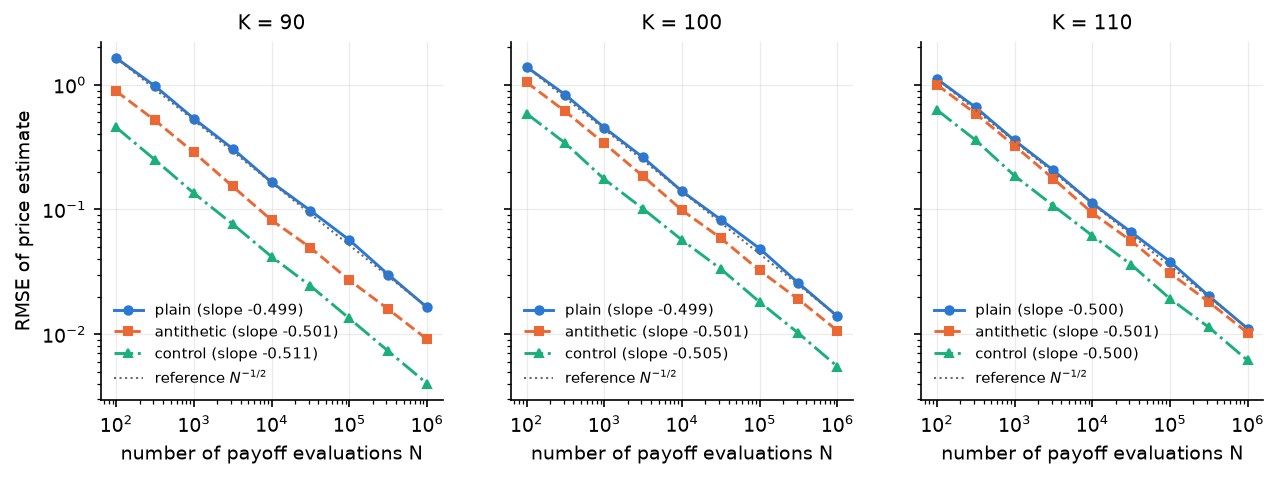
\includegraphics[width=0.5\linewidth]{fig1_rmse_vs_N.png}\caption{E1: RMSE of the MC price against $N$ (log--log), 400 replications; slopes in the legend.}\label{f1}\end{figure}
\emph{Why do control variates beat antithetic variates?} The variance ratios are $1/(1-\rho^2)$ (control; $\rho$ = payoff--stock correlation) and $1/(1+\rho_a)$ (antithetic; $\rho_a=\mathrm{corr}(Y(Z),Y(-Z))$). We measure $\rho=\rhoCtlA,\rhoCtlB,\rhoCtlC$ and $\rho_a=-\rhoAntA,-\rhoAntB,-\rhoAntC$ for $K=90,100,110$, which reproduces Table~\ref{t1}. The payoff is linear in the stock above $K$, so the stock explains most of it, whereas the mirror trick only uses the symmetry of $Z$; gains fall out of the money (\pzeroC\% of payoffs are zero at $K=110$). Antithetic costs about half the CPU time, the control variate about $1.4\times$; cost-adjusted, control wins clearly at $K=90$ (\caCvA\ vs.\ \caAntA), narrowly at $K=100$ (\caCvB\ vs.\ \caAntB) and ties at $K=110$ (\caCvC\ vs.\ \caAntC).

\textbf{E2/E4: how does the hedging error depend on $M$, and does theory predict it? (Fig.~\ref{f2}, Table~\ref{t2})} The error is centred near zero and its sd falls steadily: for $K=100$ from \sdFourB\ ($M=4$) to \sdFiveOhFourB\ ($M=504$), a tenfold fall for a 126-fold increase in $M$. Under $Q$ the mean of $HE_M$ is statistically zero in all \nconf\ configurations (largest $|z|=\maxz$, below the Bonferroni 5\% threshold \bonf). The summed formula (12) matches the simulation within 0.1--2.5\% for $M\ge126$.
\begin{table}[!htbp]\centering\small
\begin{tabular}{rrrrrrr}\toprule
 & \multicolumn{4}{c}{sd$(HE_M)$, $\mu=r$} & \multicolumn{2}{c}{mean $(\times10^{-3})$ (SE), $K=100$}\\\cmidrule(lr){2-5}\cmidrule(lr){6-7}
$M$ & $K{=}90$ & $K{=}100$ & theory (12), $K{=}100$ & $K{=}110$ & $\mu=r$ & $\mu=0.15$\\\midrule
4 & 2.357 & 3.061 & 2.885 & 3.293 & $-6.0\,(9.7)$ & $-241.0\,(9.6)$ \\
12 & 1.433 & 1.826 & 1.762 & 1.958 & $-13.0\,(5.8)$ & $-80.9\,(5.5)$ \\
26 & 0.986 & 1.263 & 1.230 & 1.354 & $+8.2\,(4.0)$ & $-29.8\,(3.8)$ \\
52 & 0.709 & 0.900 & 0.886 & 0.962 & $+6.2\,(2.8)$ & $-11.8\,(2.7)$ \\
126 & 0.464 & 0.586 & 0.578 & 0.626 & $-1.6\,(1.9)$ & $-7.0\,(1.8)$ \\
252 & 0.327 & 0.415 & 0.412 & 0.446 & $-1.2\,(1.3)$ & $-5.1\,(1.2)$ \\
504 & 0.230 & 0.295 & 0.293 & 0.313 & $+0.4\,(0.9)$ & $-1.1\,(0.9)$ \\\\\bottomrule\end{tabular}
\caption{E2/E3 ($\sigma=0.2$, $10^5$ paths): standard deviation and mean of $HE_M$; ``theory'' is the exact sum version of (12).}\label{t2}\end{table}
\begin{figure}[!htbp]\centering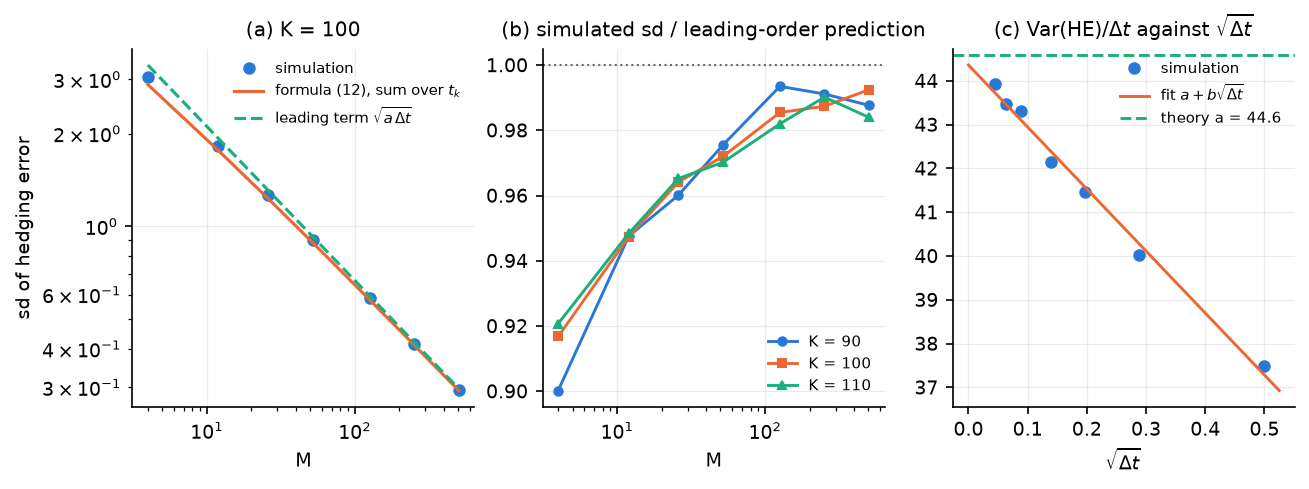
\includegraphics[width=0.5\linewidth]{fig6_theory_vs_sim.png}\caption{E2/E4 ($\mu=r$, $\sigma=0.2$): (a) sd and theory, $K=100$; (b) sd over leading term $\sqrt{a\Delta t}$; (c) $\Var/\Delta t$ against $\sqrt{\Delta t}$, fit $a+b\sqrt{\Delta t}$ (orange), theoretical $a$ (dashed).}\label{f2}\end{figure}
\emph{The strict slope criterion fails.} We pre-specified that $M^{-1/2}$ is confirmed if the bootstrap interval of the slope for $M\ge52$ contains $-\tfrac12$. It does not: for $K=100$ the slope is \slopeHiB\ with interval [\slopeHiLoB, \slopeHiHiB] ($\slopeHiA$ and $\slopeHiC$ for $K=90,110$). Theory explains this: $b<0$ ($b=\bFitB$, Fig.~\ref{f2}c), so the local slope is shallower than $-\tfrac12$ and approaches it slowly; Fig.~\ref{f3}c shows the summed theory moving from \lsThFirst\ ($M=4$ to 12) to \lsThLast\ (252 to 504), with simulation at \lsSimLast. Over $M\ge52$ theory gives \thSlopeHiB: the law holds asymptotically, not as a strict power law. The fitted constants agree with theory for $K=90$ ($a$: [\aLoA, \aHiA] vs.\ \aThA) and $K=100$ ([\aLoB, \aHiB] vs.\ \aThB) but not $K=110$ ([\aLoC, \aHiC] vs.\ \aThC, a 1.3\% gap).

\textbf{E3: how do strike, volatility and drift matter? (Fig.~\ref{f3})} We repeat E2 for three strikes, three volatilities and two drifts. \emph{Strike.} Relative to the option price the error is largest out of the money (RMSE$/C_0$ at $M=52$: \relRmseFiftyTwoA\%, \relRmseFiftyTwoB\%, \relRmseFiftyTwoC\% for $K=90,100,110$). In absolute terms it is largest at $K=110$, not at the money as we expected (sd at $M=52$: \sdFiftyTwoA, \sdFiftyTwoB, \sdFiftyTwoC). The step error is proportional to the dollar gamma $S^2\Gamma$, large when the stock is near the strike late in the option's life. Evaluating (12) over a grid of strikes (Fig.~\ref{f3}a) gives a smooth curve peaking at $K=\peakK$; dividing by $K$ moves the peak to $K=\peakKperK$, next to the forward price $S_0e^{rT}=\fwd$ where the stock most likely ends. The factor $S^2\propto K^2$ pushes the absolute peak higher. \emph{Volatility.} The sd is almost proportional to $\sigma$ (\sdSigLow, \sdSigMid, \sdSigHigh\ at $M=252$ for $\sigma=0.1,0.2,0.4$), because $S^2\Gamma\propto1/\sigma$ gives $a\propto\sigma^2$ in (12).
\begin{figure}[!htbp]\centering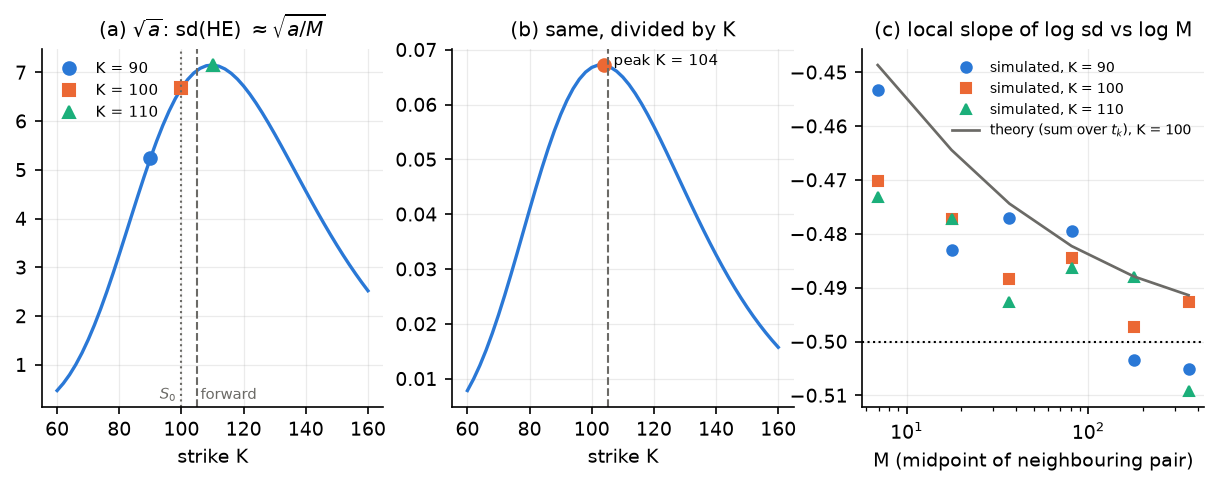
\includegraphics[width=0.5\linewidth]{fig7_strike_and_local_slopes.png}\caption{(a)--(b) Theoretical $\sqrt a$ against strike, and over $K$; (c) local slope of $\log$ sd against $\log M$ (simulation, theory).}\label{f3}\end{figure}
\emph{Drift.} Hedging never uses $\mu$, so (9) holds for any $\mu$, but the path law changes. With $\mu=0.15>r$ the discounted stock drifts upward, so the true delta tends to exceed the held $\delta_k$, giving a small negative mean error of order $\Delta t$: for $K=100$ the mean is \meanPFour\ at $M=4$ and \meanPTwoFiftyTwo\ at $M=252$ (\meanOverSdPct\% of the sd), and $M\times$mean stays between \MmeanHigh\ and \MmeanLow\ for $\sigma=0.1$ over $M\le126$. The sd shifts by factors \sdRatioPA, \sdRatioPB, \sdRatioPC\ for $K=90,100,110$ ($M\ge52$), as the stock spends more or less time near the strike; (12) with drift $\mu$ predicts these within 1--6\%.
\begin{figure}[!htbp]\centering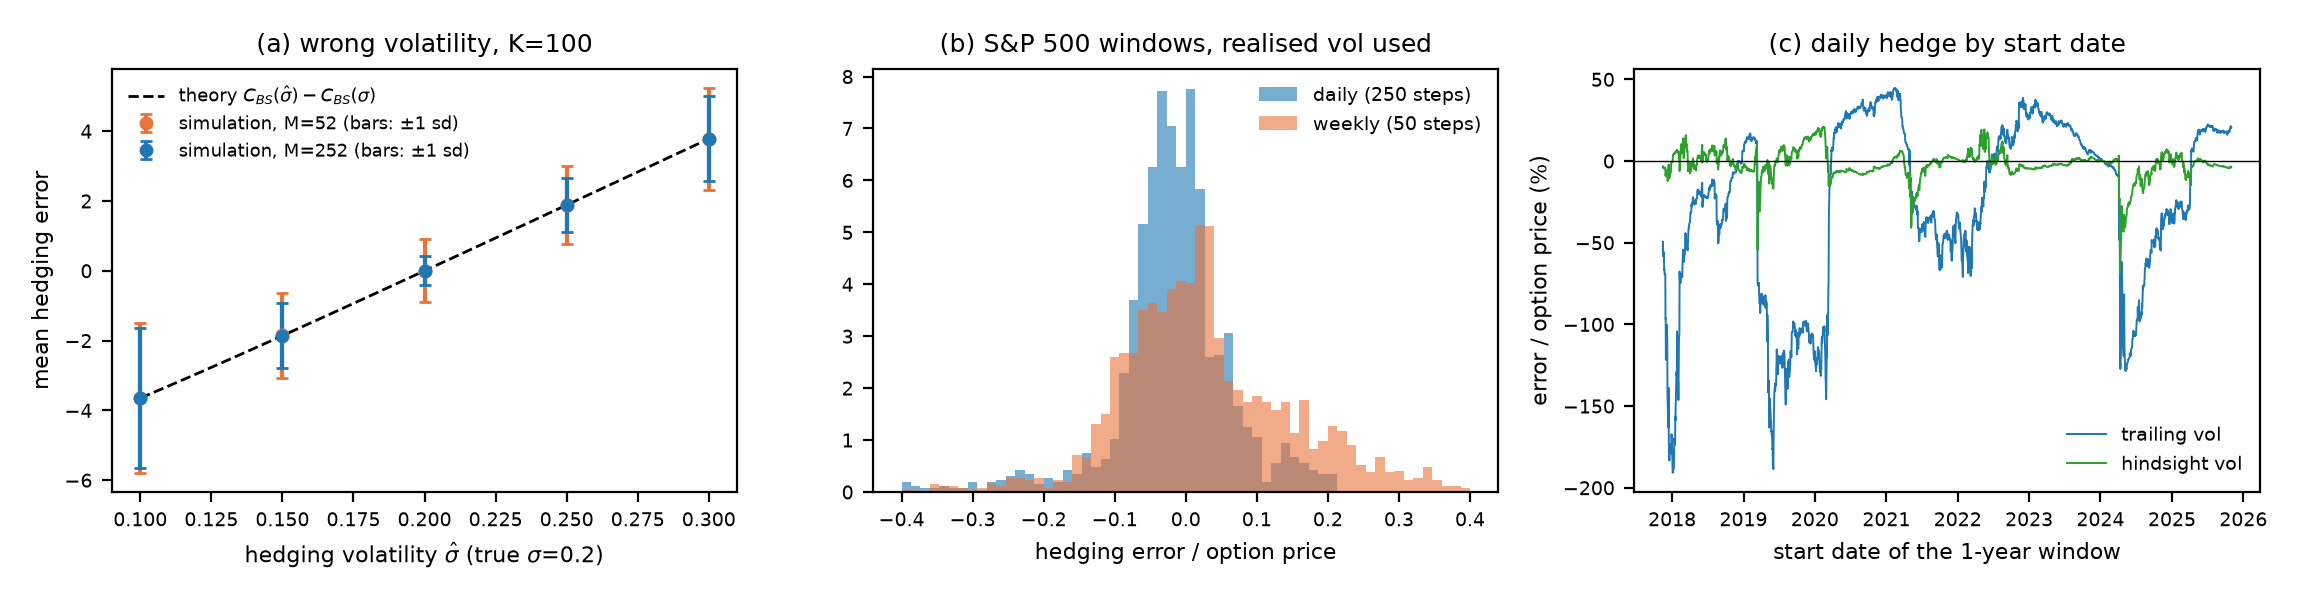
\includegraphics[width=0.75\linewidth]{fig9_wrong_vol_and_real_data.png}\caption{E5/E6: (a) mean error against hedging volatility $\hat\sigma$ ($K=100$, bars $\pm1$ sd) with theory; (b) S\&P~500 windows, daily vs.\ weekly $HE/C_0$ (realised volatility); (c) daily-hedge error by start date, trailing vs.\ realised volatility.}\label{f5}\end{figure}

\textbf{E5/E6: wrong volatility and real data (Fig.~\ref{f5}).} \emph{Wrong volatility.} Hedging with $\hat\sigma\ne\sigma=0.2$ adds, by It\^o on $e^{-rt}C(t,S;\hat\sigma)$, the term $\frac12(\hat\sigma^2-\sigma^2)\int_0^Te^{-rt}S_t^2\hat\Gamma\,dt$ to $HE_M$; its mean equals the premium mis-pricing $C_{BS}(\hat\sigma)-C_{BS}(\sigma)$ and \emph{does not shrink with $M$}. Simulation ($K=100$, $M=252$): \wvSimHigh\ for $\hat\sigma=0.3$ (theory \wvThHigh), \wvSimLow\ for $\hat\sigma=0.1$ (theory \wvThLow), within \wvMaxRelGap\%; the bias is \wvRatioHigh\ times the sd, about \wvRelHigh\% of $C_0=\wvCzero$. \emph{Real data.} On each of \rwN\ one-year windows of S\&P~500 closes (\spStart--\spEnd; $\hat\sigma=\spVol$\%, excess kurtosis \spKurt) we sell an at-the-money call ($r=3\%$ assumed) and delta-hedge. With the volatility realised in the window, sd$(HE/C_0)$ is \rwSdDailyHind\% daily and \rwSdWeeklyHind\% weekly (GBM simulation: \rwSdDailySim\%, \rwSdWeeklySim\%); the weekly/daily ratio is \rwRatioReal, not $\sqrt5=\rwRatioTheory$ (simulation \rwRatioSim): volatility changes and jumps dominate discretisation. With the trailing one-year volatility the sd is \rwSdDailyTrail\% (\rwRatioDailyHindVsTrail$\times$ larger) as regimes shift (e.g.\ 2020): E5's bias at work. Windows overlap ($\approx8$ independent years), so this is descriptive (block-bootstrap intervals in \texttt{results/e8\_real\_data\_summary.csv}).

\section{Discussion and conclusion}
The two convergences are separate. MC pricing error falls like $N^{-1/2}$ (slopes $-0.50\pm0.01$) and variance reduction changes only the constant: the control variate cut the variance by a factor of \vrCvC--\vrCvA\ depending on strike. Hedging error falls like $M^{-1/2}$ only asymptotically (slope $\approx-0.49$ for $M\ge52$) and is independent of $N$; halving it needs four times the trades, and even $M=252$ leaves \relRmseTwoFiftyTwoB\% of $C_0$ at the money and \relRmseTwoFiftyTwoC\% out of the money. Theory (12) predicts the size within 2.5\% for $M\ge126$ and explains the strike, volatility and drift effects. A wrong volatility adds a bias that rebalancing cannot remove; on real data this dominates. \textbf{Limitations:} constant $\sigma$ and $r$; no transaction costs; one option; $10^5$ paths, 400 replications (sd noise about 0.5\%, RMSE about 3.5\%); first-order asymptotics; exact premium and $\Delta$; real data from one index, overlapping windows, assumed $r$.

\begin{thebibliography}{9}\footnotesize\setlength{\itemsep}{0pt}
\bibitem{bs} F. Black and M. Scholes, The pricing of options and corporate liabilities, \emph{J. Political Economy} 81 (1973), 637--654.
\bibitem{be} P. Boyle and D. Emanuel, Discretely adjusted option hedges, \emph{J. Financial Economics} 8 (1980), 259--282.
\bibitem{bkl} D. Bertsimas, L. Kogan and A. Lo, When is time continuous?, \emph{J. Financial Economics} 55 (2000), 173--204.
\bibitem{gl} P. Glasserman, \emph{Monte Carlo Methods in Financial Engineering}, Springer, 2004.
\bibitem{fred} FRED, Federal Reserve Bank of St.\ Louis, series SP500 (S\&P 500 daily close), \texttt{fred.stlouisfed.org/series/SP500}.
\bibitem{sh} S. Shreve, \emph{Stochastic Calculus for Finance II}, Springer, 2004.
\end{thebibliography}
\end{document}
